\documentclass[a4paper]{scrartcl}
\usepackage[utf8]{inputenc}
\usepackage{xcolor}
\usepackage{graphicx}
\graphicspath{ {./figure/} }

\title{Assignment 1}
% \textcolor{gray}{Critique and re-design of an existing graphic}
\author{Alina Mokrova\\
				id
				\and
				Levente	Slajchó\\
				id
				\and
				Maximilian Walterskirchen\\
				id
				\and
				Leminh Nguyen\\
				11945068}
\date{\today}

\begin{document}

\maketitle

\section{Analysis and criticism}

%     \item In a first step you should argue why the given presentation is not
%       appropriate to represent the data in an efficient way. Please argue about
%       the deficiencies of the graphic with respect to the design principles we
%       covered in the lecture (Data-Ink-Ratio, Visual Clutter, ...).  Hand in a
%       short text about your argumentation.

% \textcolor{gray}{To deal with a given static graphic, to identify deficiencies
% of the visual representation, and to find a more suitable way to present the
% data at hand.}

\subsection{Analysis of this graphic}

    % \begin{itemize}
    %    \item Nutritional comparison between processed and natural/wholesome food
    %    \item Comparisons:
    %    \begin{itemize}
    %      \item Cost per calorie
    %      \item Calories per 100g
    %      \item Sugar per 100g
    %      \item A pack of chips is more energy dense than compared to an apple
    %      \item Wholesome food is more expensive, the ratio of value to calorie for an apple is higher as for a bag of potato chips
    %    \end{itemize}
    %    \item Suggestions of the infographic:
    %    \begin{itemize}
    %        \item Stick to the periphery of the supermarket to find the natural food
    %        \item Processed foog containing the most calories by weight are located at the center of the grocery store
    %    \end{itemize}
    %    \item 
    % \end{itemize}

\subsection{Criticism of the visual design}

In this section, the three sub-infographics will be criticised according to the information design cues from the lecture notes.

% Some notes:
% \begin{itemize}
%     \item The author uses the \textit{Bottom up} approach which is data driven
%     \item The graphics is a conventional representation an used the controlled visualization paradigm (reason: data driven)
%     \item Which requires the attentive perception of the reader/viewer
%     \item Attentive approach is slow to perceive and easy to forget information
%     \item Based on visual processing paradigm and requires the following from the viewer:
%     \begin{itemize}
%         \item Parallel processing to extract low level properties of the visual scene
%         \item Pattern perception
%     \end{itemize}
%     \item Deficiency for viewers with color blindness, see produce aisle/section which is represented in red and green
%     \item Graphic in 3 dimensions which makes it way more complex than it is
%     \item The food graphical components obscure the actual information and data $\rightarrow$ hard to perceive actual infographic
%     \item Preattentive processing:
%     \begin{itemize}
%         \item No immediate understanding
%         \item No preattentive attributes except for food labels, but many are obscured by other components
%         \item Hard for immediate perception
%     \end{itemize}
%     \item The perspective suggests the entry of the store in the graphic is on the right side, and that the higher numbers of the table are closer in perspective $\rightarrow$ based on the western left to right reading perspective it should be the other way around
%     \item The differences between the three tables are difficult to compare due to too much information and bright color
%     \item Data-Users-Tasks triangle:
%     \begin{itemize}
%         \item Expressiveness - Are the visual elements expressive enough? $\rightarrow$ Even too much
%         \item Effectiveness - Is the information displayed effectively? $\rightarrow$ Not at all
%         \item Appropriateness - Is the visualization appropriate? $\rightarrow$ Yes, it's perfect for the subject
%     \end{itemize}
% \end{itemize}

\section{Assessment of redesign}

%     \item In a third step you should argue why you chose to represent the data
%       that way. What did you change? Why is this representation better suited
%       than the original one? Hand in a short text about your argumentation.

% link to appendix of new design

\bibliographystyle{unsrt}
\bibliography{ivassignment}

\newpage
\clearpage
\section{Appendix}

\begin{figure}[h]
  \centering
	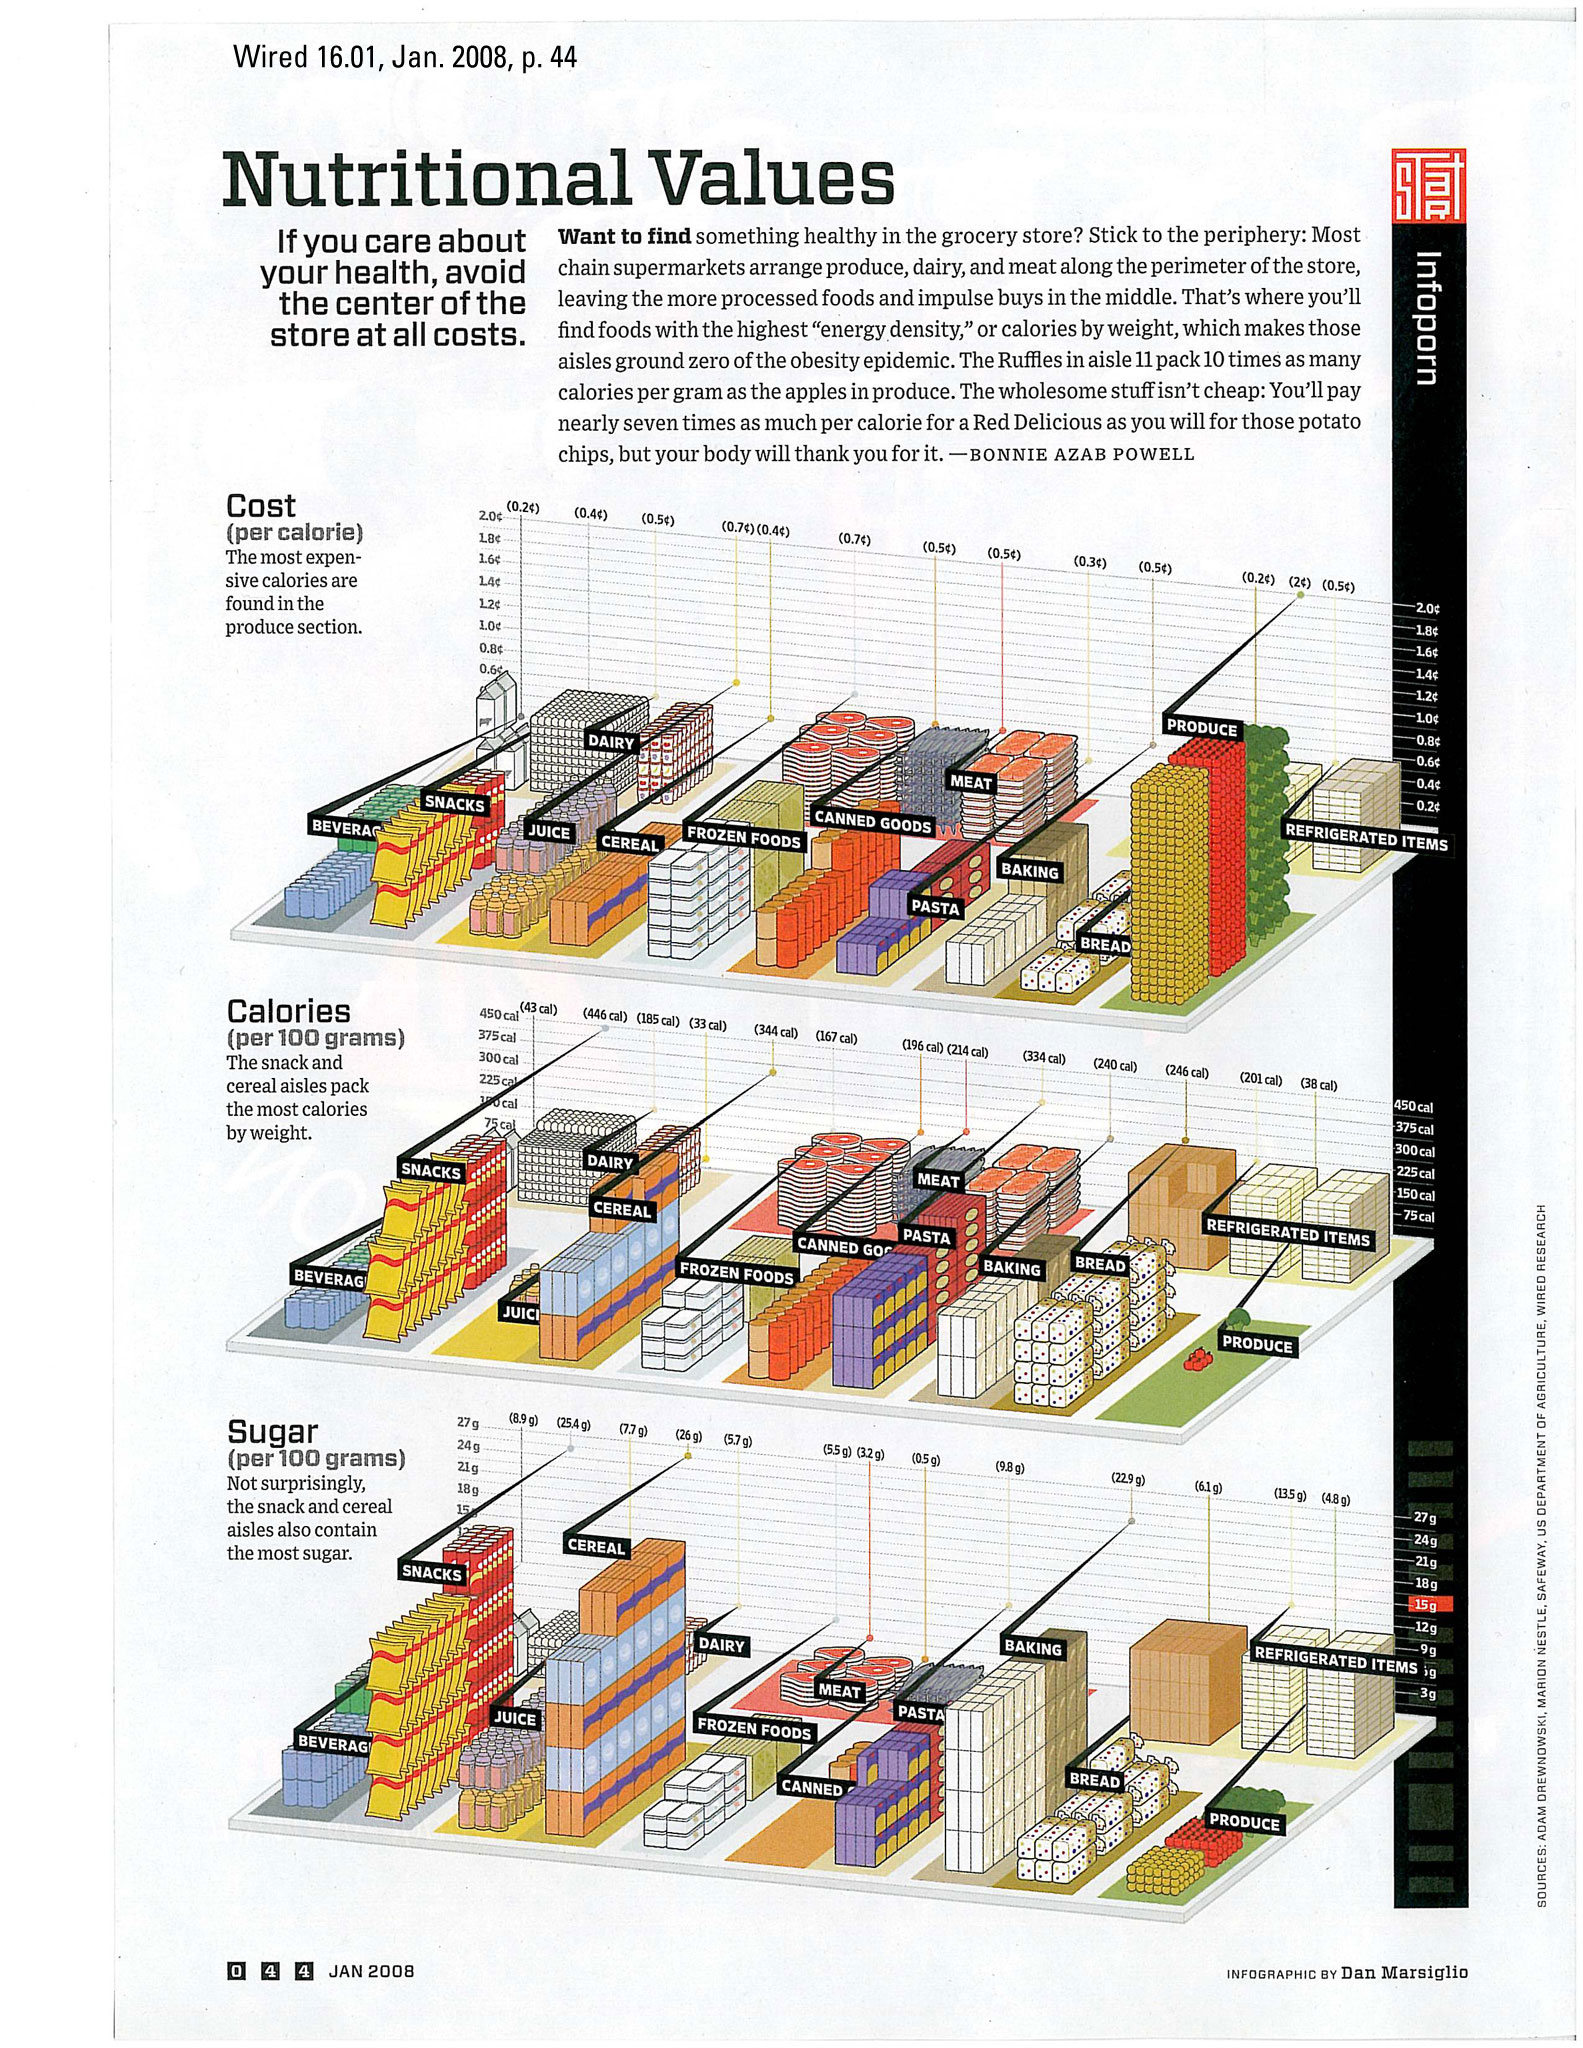
\includegraphics[scale=0.20]{figures/assignmentGraphic.jpg}
  \label{assignmentGraphic}
  \caption{Given graphic to criticize.}
\end{figure}

\end{document}
